\documentclass[conference]{IEEEtran}
\IEEEoverridecommandlockouts
% Ported from docs/SCIS-ISIS_paper/IEEEconference-latex-template/paper_draft.md
% (Sections I-V are the user-signed-off text, converted verbatim to LaTeX).
% Section VI carries measured E0/E1/E1b/E3 data (as of 2026-07-16); E4/E5/E6 are
% marked PENDING per the project's "never fabricate a number" rule -- fill in from
% docs/experiment_results.md as those experiments complete.
% Abstract, Keywords, and Section VII are DRAFT ONLY and still need user sign-off,
% consistent with docs/SCIS-ISIS_paper/IEEEconference-latex-template/paper_draft.md's
% "only paragraphs the user has signed off on" rule.

\usepackage{cite}
\usepackage{amsmath,amssymb,amsfonts}
\usepackage{algorithmic}
\usepackage{graphicx}
\usepackage{textcomp}
\usepackage{xcolor}
\usepackage{tikz}
\usetikzlibrary{positioning,calc,arrows.meta}
\def\BibTeX{{\rm B\kern-.05em{\sc i\kern-.025em b}\kern-.08em
    T\kern-.1667em\lower.7ex\hbox{E}\kern-.125emX}}

% --- Draft-only helpers: remove before camera-ready ---
\newcommand{\TODO}[1]{\textcolor{red}{[TODO: #1]}}
\newcommand{\FIGPLACEHOLDER}[2]{%
  \fbox{\begin{minipage}[c][#1][c]{\linewidth}\centering\footnotesize TODO figure asset --- #2\end{minipage}}%
}

\begin{document}

\title{Energy-Aware Arm and Base Selection for a Dual-Gantry Quad-Arm Ceiling Robot Using a GNG Capability Map}

\author{
\IEEEauthorblockN{1\textsuperscript{st} Raditya Artha Rochmanto\textsuperscript{1,2}}
\IEEEauthorblockA{\textsuperscript{1}\textit{Department of Mechanical Systems Engineering, Graduate School of Systems Design} \\
\textit{Tokyo Metropolitan University}\\
6-6 Asahigaoka, Hino, Tokyo 191-0065, Japan \\
rochmanto-artha@ed.tmu.ac.jp}
\IEEEauthorblockA{\textsuperscript{2}\textit{Department of Electrical Engineering} \\
\textit{Politeknik Negeri Semarang}\\
Indonesia}
\and
\IEEEauthorblockN{2\textsuperscript{nd} Anhar Risnumawan\textsuperscript{1,2}}
\IEEEauthorblockA{\textsuperscript{1}\textit{Department of Mechanical Systems Engineering, Graduate School of Systems Design} \\
\textit{Tokyo Metropolitan University}\\
6-6 Asahigaoka, Hino, Tokyo 191-0065, Japan \\
risnumawan-anhar@ed.tmu.ac.jp}
\IEEEauthorblockA{\textsuperscript{2}\textit{Mechatronics Engineering Division} \\
\textit{Politeknik Elektronika Negeri Surabaya}\\
Indonesia}
\and
\IEEEauthorblockN{3\textsuperscript{rd} Achmad Fahrul Aji\textsuperscript{1,2}}
\IEEEauthorblockA{\textsuperscript{1}\textit{Department of Mechanical Systems Engineering, Graduate School of Systems Design} \\
\textit{Tokyo Metropolitan University}\\
6-6 Asahigaoka, Hino, Tokyo 191-0065, Japan \\
achmad-aji@ed.tmu.ac.jp}
\IEEEauthorblockA{\textsuperscript{2}\textit{Department of Electrical Engineering} \\
\textit{Politeknik Negeri Semarang}\\
Indonesia}
\and
\IEEEauthorblockN{4\textsuperscript{th} Naoyuki Kubota}
\IEEEauthorblockA{\textit{Department of Mechanical Systems Engineering, Graduate School of Systems Design} \\
\textit{Tokyo Metropolitan University}\\
6-6 Asahigaoka, Hino, Tokyo 191-0065, Japan \\
kubota@tmu.ac.jp}
}

\maketitle

\begin{abstract}
% DRAFT -- not yet signed off; follows the "Approach and contributions" (I-¶4) and
% "Results preview" (I-¶5) paragraphs below.
The two ceiling-mounted \textcolor{red}{rails} carrying four arms \textcolor{red}{turn} every pick into two coupled decisions:
which arm should act, and where \textcolor{red}{its base should go}, since repositioning the
\textcolor{red}{base} is one of the dominant costs of the motion. We propose an energy-aware
selection cost $J$ that chooses the arm and the full eight-degree-of-freedom (8-DOF)
configuration together over a base-aware capability map built with Growing Neural
Gas (GNG). Every map node stores a representative configuration \textcolor{red}{that includes its rail placement}, together with its
manipulability, so \textcolor{red}{each node already fixes both an arm and a base rather than marking only whether a cell is reachable}. Treating the rail as a
degree of freedom when building the map, rather than sampling the arm alone, enlarges
the measured reachable workspace by \textcolor{red}{about four times}, and a boundary-seeding step
keeps the map accurate to within a few centimetres of the true reach surface. In
simulation on NVIDIA Isaac Sim, \textcolor{red}{energy-aware
selection is evaluated} against \textcolor{red}{nearest, fixed, and random baseline} policies for
arm and base choice, using a rail dynamics model with an assumed Coulomb/viscous
friction (a modelling assumption, not measured hardware data) so that
repositioning the rail carries a real energy cost; \textcolor{red}{over a
60-position grid, the multi-arm policies (energy-aware, nearest, random) each
reach 93.3\% plan success, versus 63--65\% for any single fixed arm, and
energy-aware selection reaches the lowest mean measured mechanical energy of the
three multi-arm policies (5.1\% below nearest, 3.1\% below random), with a
majority (57--61\%) same-target pairwise win rate against each baseline, though
the median result is closer -- a real but partial improvement, not a uniform win
on every metric}.
\end{abstract}

\begin{IEEEkeywords}
mobile manipulation, capability map, growing neural gas, redundant manipulator,
base placement, energy-aware planning
\end{IEEEkeywords}

\section{Introduction}

\textcolor{red}{An aging global population is driving demand for assistive robots that
can operate inside the home \cite{unitednations2024world,who2025clinical}, taking on
tasks such as retrieving objects, tidying, and delivering items to occupants
\cite{IFR2025,Lisondra2026}. Residential deployment is harder than factory or outdoor
use \cite{kemp2007challenges}: homes are small and cluttered, and a floor-traversing
mobile manipulator shares that space with residents, who must stay alert to avoid it
\cite{sisbot2007human}. Lifting the robot off the floor entirely \cite{Lalonde2025}
removes this conflict -- a ceiling-mounted arm keeps the floor free while still
serving as an in-home assistant from above \cite{Kaluarachchi2025}. We study such a
ceiling robot: a dual-gantry system in which each gantry carries two 6-DOF arms,
forming a quad-arm cooperative overhead manipulator.}

\textcolor{red}{Each gantry moves both linearly and rotationally, giving each arm 8~DOF
in total. Most objects are reachable by several arms from a range of base positions,
so the robot faces two coupled questions: which arm should act, and where should its
base be positioned first? Both are costly -- repositioning the heavy base costs time
and energy \cite{MoMaPos2024,BaSeNet2024,EnergySLR2024} -- and naive policies (nearest
arm, or leaving the base where it is) can waste base travel. We address the problem
of selecting the arm and base placement that minimizes energy.}

\textcolor{red}{Reachability and capability maps are the standard tool for depicting an
arm's reachable regions and mobility, and for placing a robot optimally
\cite{Zacharias2007,Makhal2018}, but two assumptions limit them here. Most are built
for a fixed base, so they miss the reachable space a mobile base opens up; and they
typically record only whether a cell is reachable, not the cost of reaching it or an
IK-ready configuration \cite{Zacharias2007}. Recent work improves operator awareness
of obstacles and nearby objects \cite{MoMaPos2024,InvReach2022}, and
redundancy-resolution methods optimize a single arm's posture for manipulability
\cite{Yoshikawa1985}, but neither selects between multiple arms nor accounts for the
base's own cost. What is missing is a representation that answers, directly, which
arm and which base placement minimize energy on a ceiling-rail robot.}

\textcolor{red}{We address this with an energy cost $J$ that operates on a base-aware
capability map built with Growing Neural Gas (GNG) \cite{Fritzke1995}: each node
stores a representative 8-DOF configuration and its manipulability
\cite{Yoshikawa1985}, so a node is a full configuration -- rail placement included --
not just a reachable point. This paper makes three contributions. First, the
energy-aware selection cost $J$, which chooses the arm and the full 8-DOF
configuration (rail travel included) rather than settling for the nearest reachable
pose. Second, the base-aware GNG capability map itself, which treats the ceiling rail
as a genuine DOF and attaches a representative configuration and manipulability value
to every node, with boundary-seeding preserving accuracy at the workspace edge.
Third, an evaluation in Isaac Sim that characterizes the map, measures how much the
rail DOF expands the reachable workspace, and compares energy-aware selection against
nearest, fixed, and random baselines. Open-vocabulary perception with YOLOE supplies
the target objects the selection pipeline acts on \cite{Wang2025}.}

\textcolor{red}{Our simulation results support each claim. Treating the rail as a DOF
expands the reachable workspace roughly $4\times$ over an arm-only baseline, and
boundary-seeding recovers the true reach at the workspace edge to within about one
centimeter of the forward-kinematics surface. Energy-aware selection, alongside the
other multi-arm baselines, raises plan success from 63--65\% (any single fixed arm)
to 93.3\%; under a rail-dynamics model with assumed Coulomb/viscous friction (a
modelling assumption, not measured hardware data, so rail travel carries a real
energy cost), it also attains the lowest mean measured mechanical energy of the
three multi-arm policies (45.84~J mean vs.\ 48.28~J nearest, $-5.1\%$, and 47.31~J
random, $-3.1\%$; a majority same-target pairwise win rate of 57--61\% against each
baseline, though the median result is closer to random's -- see Section~VI-C for the
full, honestly-reported comparison). We ground these results by modeling NVIDIA
Isaac Sim \cite{IsaacSim2026} as a high-fidelity digital twin of our physical trailer
living laboratory and ceiling-mounted robot system \cite{Kubota2022}; physical
integration and real-world validation are future work, but both the trailer lab and
the ceiling hardware already exist in our facility, supporting the feasibility of
transferring the simulated controller.}

\textcolor{red}{The rest of the paper is organized as follows. Section~II reviews
related work; Section~III describes the system; Section~IV presents the base-aware
GNG capability map; Section~V defines the energy cost $J$ and the selection
procedure; Section~VI reports experiments; Section~VII concludes.}

\section{Related Work}

\noindent\textit{Reachability and capability maps.}
\textcolor{red}{A workspace can be discretized into cells and each cell labelled with
whether the end effector can reach it. Zacharias et al.\ extended this to a
capability map that also captures reach orientation, richer than a binary occupancy
grid \cite{Zacharias2007}. Reuleaux inverted the reachability map for base placement,
letting the robot pick a standing position for a target \cite{Makhal2018}. Recent
work targets construction and query cost: RM4D reduces the discretization from six
dimensions to four and serves both reachability and inverse-reachability from one
structure \cite{RM4D2024}. All of these are built for a single arm on a stationary
base, storing one reachability bit per cell. Our map differs on both counts: the
ceiling rail is a first-class part of the configuration, so it records how base
motion extends reach, and every node carries a representative 8-DOF configuration
(rail placement included) and a manipulability value, not a single bit.}

\noindent\textit{Base placement for mobile manipulators.}
\textcolor{red}{Where a mobile base should stop before manipulating is a well-studied
problem. Sandakalum et al.\ learn an inverse-reachability network that places the
platform for a task while accounting for obstacles \cite{InvReach2022}. MoMa-Pos
optimizes base placement from the kinematics of the objects to manipulate
\cite{MoMaPos2024}, and BaSeNet plans a sequence of base poses so a robot can pick up
multiple objects in succession \cite{BaSeNet2024}. This line of work is thorough on
placing a single arm well, but none of it chooses \emph{among} several arms or scores
candidate placements by the energy needed to reach them -- the gap our work fills for
a redundant ceiling-rail robot.}

\noindent\textit{Redundancy resolution and inverse kinematics.}
\textcolor{red}{A kinematic chain with more joints than the task strictly needs can use
the spare freedom for a secondary objective; Yoshikawa's manipulability measure is
the classic choice, steering a redundant arm away from singular postures
\cite{Yoshikawa1985}. Learning-driven IK has since produced solvers such as
IKDiffuser, which generates configurations with a diffusion model
\cite{IKDiffuser2025}. Each of these optimizes the posture of a single, already-chosen
arm for one criterion -- none decides which of several limbs should act, or accounts
for the base travel a given posture would require. We keep the IK solver standard and
classical, and instead use the capability map to enumerate candidate 8-DOF
configurations, each with its own arm and rail placement, which the energy cost then
ranks to settle both the arm choice and the base motion.}

\noindent\textit{Multi-arm coordination.}
\textcolor{red}{Distributing tasks across multiple arms is a related concern; recent
planners such as DAG-Plan and RoboPARA build dependency graphs over tasks and
allocate subtasks to each arm so multiple arms can work in parallel
\cite{DAGPlan2024,RoboPARA2026}. Their focus is the temporal and logical structure of
a multi-step task. Ours is different and complementary: for a single reaching action,
we ask which arm reaches the target for the least energy -- arms sharing a rail share
one moving base, while arms on different rails move independently -- and answer it
with the same map and cost that also place the base.}

\section{System}

\begin{figure*}[t]
\centering
\begin{minipage}{0.34\textwidth}\centering
  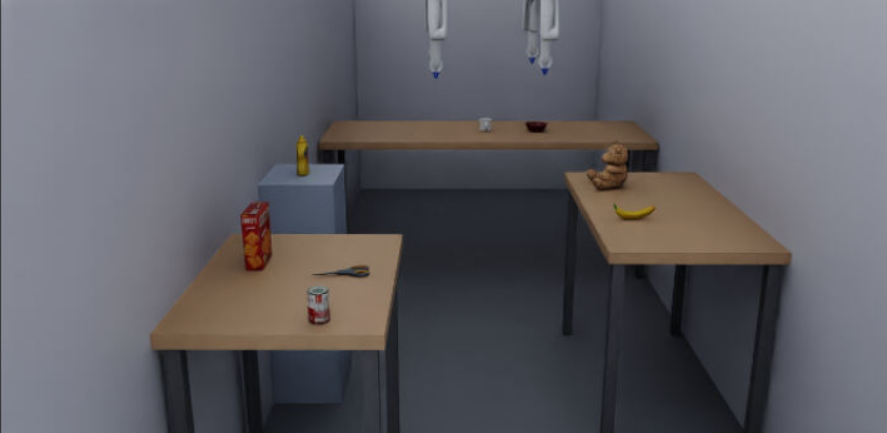
\includegraphics[width=\linewidth]{figure/Env_Isaac.png}\\
  {\footnotesize (a) system and workspace}
\end{minipage}\hfill
\begin{minipage}{0.63\textwidth}\centering
  \resizebox{\linewidth}{!}{%
  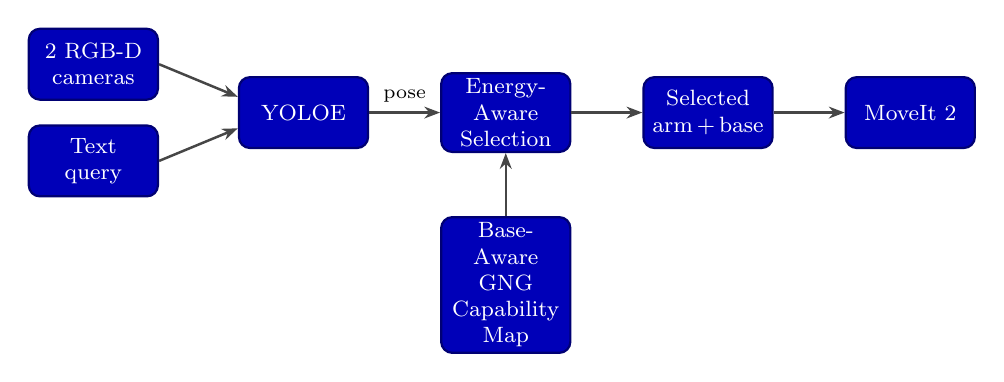
\begin{tikzpicture}[>=Stealth, thick, font=\footnotesize,
    box/.style={draw=blue!45!black, fill=blue!72!black, text=white, rounded corners,
                align=center, minimum height=9mm, text width=15mm, inner sep=2pt},
    arr/.style={-{Stealth[length=2mm]}, line width=0.9pt, draw=gray!55!black}]
    \node[box] (cam) {2 RGB-D\\cameras};
    \node[box, below=3mm of cam] (query) {Text\\query};
    \coordinate (m) at ($(cam.east)!0.5!(query.east)$);
    \node[box, right=10mm of m, anchor=west] (yolo) {YOLOE};
    \node[box, right=9mm of yolo] (sel) {Energy-\\Aware\\Selection};
    \node[box, below=8mm of sel] (gng) {Base-Aware\\GNG\\Capability Map};
    \node[box, right=9mm of sel] (arm) {Selected\\arm\,+\,base};
    \node[box, right=9mm of arm] (mv) {MoveIt~2};
    \draw[arr] (cam.east)   -- ([yshift=2mm]yolo.west);
    \draw[arr] (query.east) -- ([yshift=-2mm]yolo.west);
    \draw[arr] (yolo) -- node[above, font=\scriptsize, text=black] {pose} (sel);
    \draw[arr] (gng)  -- (sel);
    \draw[arr] (sel)  -- (arm);
    \draw[arr] (arm)  -- (mv);
  \end{tikzpicture}}\\
  {\footnotesize (b) end-to-end pipeline}
\end{minipage}
\caption{Overview of the \textcolor{red}{dual-gantry quad-arm ceiling} robot and the proposed pipeline.
(a) \textcolor{red}{Two rails mounted to the ceiling, each carrying two Kinova Gen3 Lite arms and each adding a
prismatic axis ($d$) and a revolute axis ($\theta$) that its two arms share}, so each
arm forms an 8-DOF chain $\mathbf{q}=[d,\theta,q_1 \ldots q_6]$;
two overhead RGB-D cameras observe the workspace. (b) The end-to-end pipeline,
from open-vocabulary perception, through energy-aware arm-and-base selection over
the base-aware capability map, to collision-free planning and execution.}
\label{fig:overview}
\end{figure*}

\subsection{Robot Platform and Kinematic Model}

The robot consists of two rails mounted to the ceiling, side by side, each carrying
two arms. Each arm is a Kinova Gen3 Lite, a six-joint manipulator with a reach of
about 0.76~m and a two-finger gripper at its wrist \cite{Kinova}, for four arms in
total. Each rail adds two more degrees of freedom that its pair of arms share, a
prismatic axis that slides the carriage horizontally and a revolute axis that rotates
it, so relative to the ground each arm forms an 8-DOF chain. We write a configuration
of one arm as $\mathbf{q} = [d,\ \theta,\ q_1,\ \ldots,\ q_6]$, where $d$ and $\theta$
are the translation and rotation of that arm's own rail, and $q_1 \ldots q_6$ the arm
joints. The kinematic tree is anchored at a fixed world frame. Each rail base is
attached to the world, each arm base to its own rail, and a tool frame at the gripper
defines the end-effector pose that the task is specified in. Because the two arms are
mounted on the same carriage, moving the rail moves both of them together, which
couples the choice of arm to the placement of the base, while arms on different rails
move independently. Fig.~\ref{fig:overview} shows the platform and its frames
alongside an overview of the end-to-end pipeline, from perception through
energy-aware selection to planning and execution.

\subsection{Simulation Environment}

All experiments in this paper are carried out in NVIDIA Isaac Sim, a GPU-accelerated
simulator with a physics engine suitable for contact-rich manipulation
\cite{IsaacSim2026,Mittal2023}. The simulated robot is built from the same URDF
description that defines the physical platform, so the kinematics and joint limits
used in simulation match the real hardware. The scene places a set of everyday
tabletop objects within the workspace, some within easy reach of several arms and at
least one deliberately positioned near the edge of the reachable workspace
(Fig.~\ref{fig:perception}). The scene is observed by two RGB-D cameras placed above the
workspace, which are the system's only exteroceptive sensor. Their images serve two
roles at once. The color stream feeds the object detector, and the depth stream builds
the collision octomap used for planning, so a single sensing rig supports both
perception and collision avoidance. We treat the simulator as the evaluation platform
for this work and validate on the physical robot in future work.

\subsection{Perception Front End}

The target objects are supplied to the pipeline by an open-vocabulary perception
module based on YOLOE, a real-time model that detects and segments objects
from free-form text prompts \cite{Wang2025}. \textcolor{red}{Each of the two overhead
cameras is processed independently. The colour image yields a per-object
segmentation mask; the masked pixels of the aligned depth image are back-projected
into a 3D point set, which is carried into the world frame through the fixed
camera-to-world transform. We take the \emph{median} of those world points as the
object's centroid, which rejects the depth outliers that occur along the mask
border. The two cameras' detections are then fused: two centroids that fall within
a small merge radius (0.10~m) are taken to be the same physical object, their
positions are averaged, and the higher of the two observed object tops is kept
(each camera sees only part of a top). A lightweight track layer with majority
label voting removes any remaining cross-camera duplicate and stabilises the class
label across frames. The result is a single world-frame position per named object,
robust to a partial or one-sided view, obtained without a fixed object database, so
the operator can request an object by name (Fig.~\ref{fig:perception}).} In this
context, perception functions as the enabling front end, providing the target on
which the capability map and the energy cost are subsequently based.

\begin{figure}[htbp]
\centering
\begin{minipage}{0.49\linewidth}\centering
  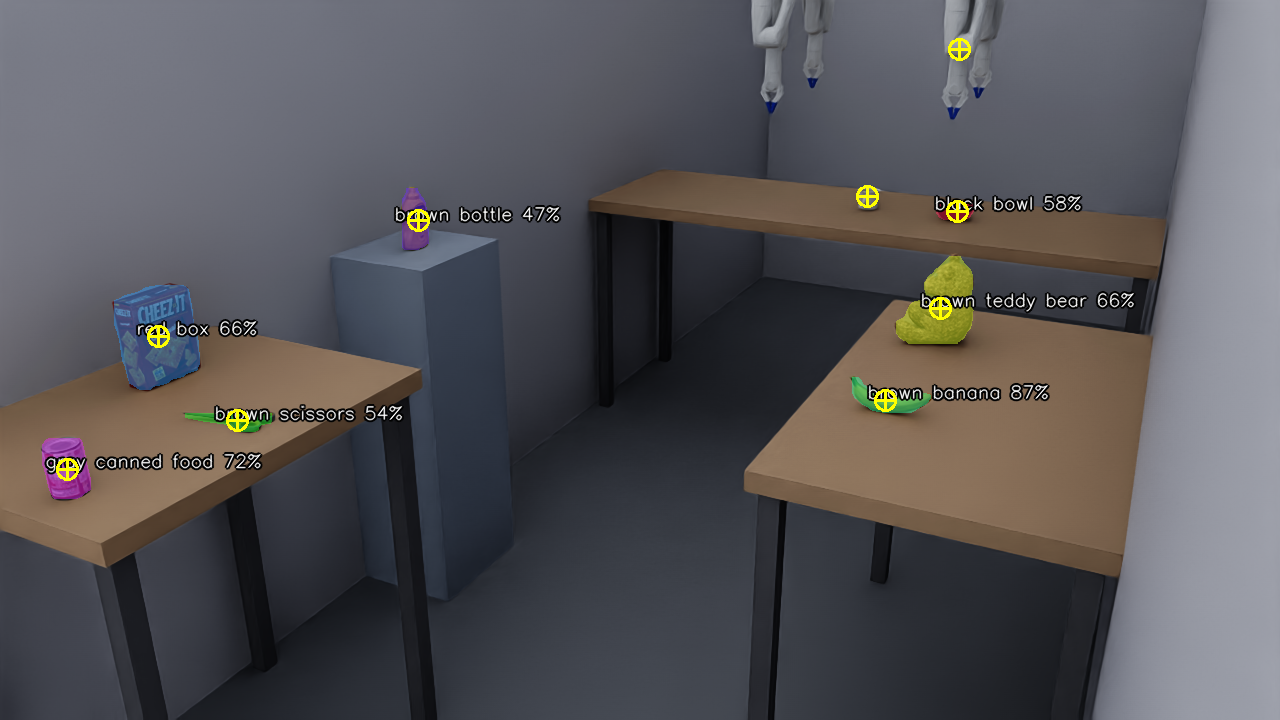
\includegraphics[width=\linewidth]{figure/perception_rgbd_20260717_162902.png}\\
  {\footnotesize (a) camera~1}
\end{minipage}\hfill
\begin{minipage}{0.49\linewidth}\centering
  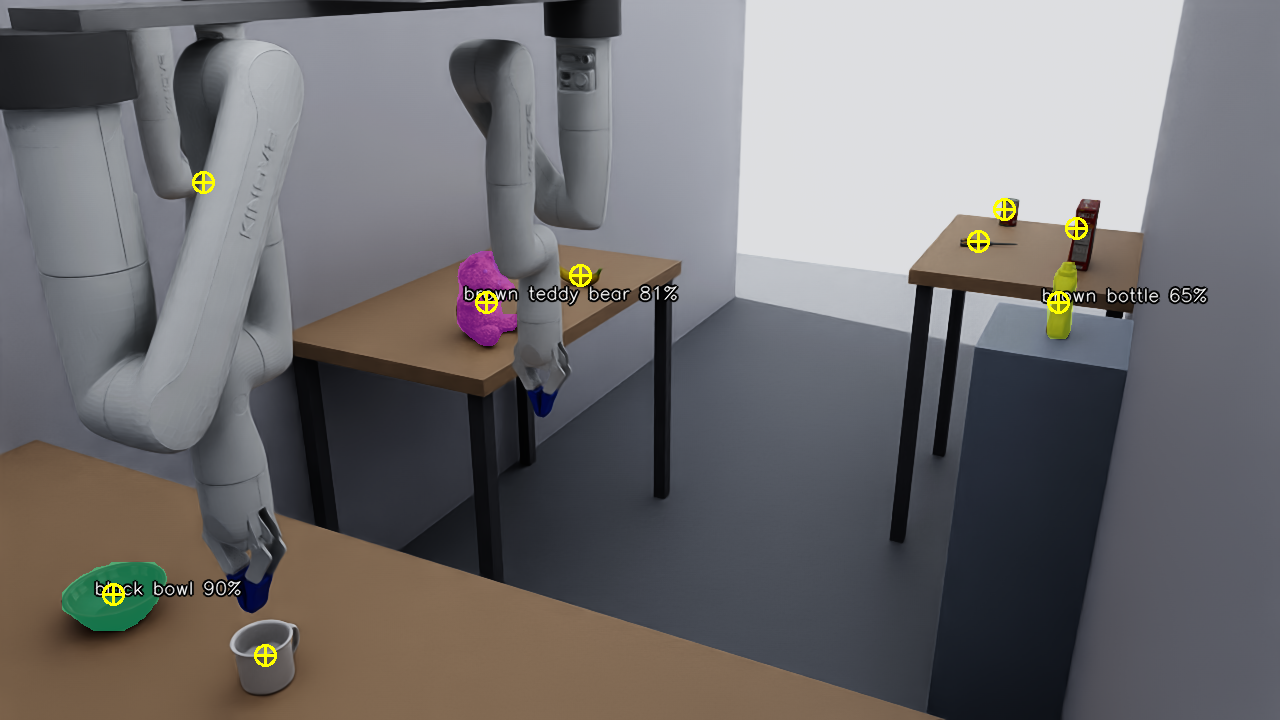
\includegraphics[width=\linewidth]{figure/perception_rgbd2_20260717_163458.png}\\
  {\footnotesize (b) camera~2}
\end{minipage}
\caption{\textcolor{red}{The simulated workspace in NVIDIA Isaac Sim and the
open-vocabulary perception, seen by the two overhead RGB-D cameras placed at the
two ends of the corridor the rails run along: (a)~camera~1 and (b)~camera~2. The
tabletop objects used in the experiments are visible, at least one near the edge of
the reachable workspace. YOLOE detects and segments each object from a text prompt
(coloured masks with class label and confidence); for every mask the aligned depth
is back-projected and its median taken as a world-frame centroid (yellow
cross-hair). Detections from the two viewpoints are fused by centroid proximity and
majority label voting, giving one localised position per named object with no fixed
object database.}}
\label{fig:perception}
\end{figure}

\subsection{Planning and Execution Stack}

\textcolor{red}{Given a target and a candidate configuration, the motion layer is
built on MoveIt~2 \cite{Coleman2014} with planners from the Open Motion Planning
Library \cite{Sucan2012}. Inverse kinematics requests are answered by MoveIt against
the current robot state, and collisions are checked against an octomap populated
from the two cameras' depth images, so a plan avoids both the scene and the robot's
own body; the object selected for removal is isolated from the octomap's source
cloud so it can be grasped, while the remaining objects and the environment stay as
obstacles. We build the capability map of Section~IV offline with the Pinocchio
rigid-body-dynamics library \cite{Carpentier2019}, which is also used for forward
kinematics when sampling configurations. At execution time, a candidate is drawn
from the map, MoveIt plans a collision-free motion to it, and the motion is executed
in simulation. Section~V covers which candidate is selected and in what order.}

\section{Base-Aware GNG Capability Map}

\textcolor{red}{Our core idea is a per-arm capability map: for each location the
end-effector can reach, the map stores a configuration that achieves it and a
quality measure for that configuration. Unlike a plain reachability map, which only
encodes whether a location is attainable, ours attaches a concrete configuration and
a quality value to every reachable location, and it is base-aware because the stored
configuration includes the rail's degrees of freedom. We build one such map per arm,
so the four arms across the two rails are described by four independently-queried
maps (Section~V).}

\subsection{Sampling Reachable Configurations}

We sample the 8-DOF configuration
$\mathbf{q} = [d,\ \theta,\ q_1,\ \ldots,\ q_6]$ uniformly within the joint limits
and compute the resulting end-effector pose by forward kinematics with the
Pinocchio library \cite{Carpentier2019}. For each sample we also record the
manipulability $w = \sqrt{\det(JJ^\top)}$ \cite{Yoshikawa1985}. This produces a dataset of
(pose, $\mathbf{q}$, manipulability) tuples that covers the combined
arm-and-rail workspace. Because the rail translation $d$ and rotation $\theta$ are
sampled alongside the arm joints, the dataset already reflects the reach that base
motion provides, not just the reach of a fixed arm.

\subsection{Growing the Map}

We fit a Growing Neural Gas network \cite{Fritzke1995} to this dataset. Each node
stores a vector $[\mathbf{x} \mid \mathbf{q}]$ that concatenates the end-effector
position $\mathbf{x}$, which we call the task part, with the configuration
$\mathbf{q}$ that produces it. Training is arranged so that the best-matching-unit
search uses the task part alone, which makes the nodes tile the reachable
workspace, while adaptation updates the whole vector, so each node's $\mathbf{q}$
converges to a configuration that is representative of its workspace cell. Edges
are formed between co-activated nodes by competitive Hebbian learning, giving the
map a topology over the workspace. Every node is therefore two things at once, a
location the end-effector can reach and a representative 8-DOF configuration that
reaches it, rail placement included. This is the sense in which the map is
base-aware. Because $\mathbf{q}$ carries the rail translation and rotation, two ways
of reaching the same point from different base placements settle into different
nodes, so a node's configuration stays a valid single posture rather than an average
of incompatible base positions. To keep the map faithful at the reachable boundary,
where nodes grown only from interior samples would otherwise settle inward, we pin a
shell of nodes on the measured reach surface before growing the interior
(Fig.~\ref{fig:gngmap}), and Section~VI reports the resulting edge fidelity.

\begin{figure}[htbp]
\centering
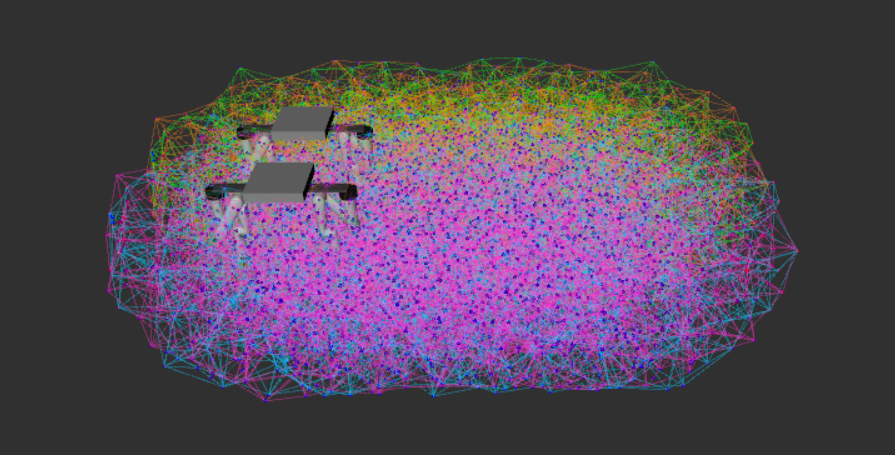
\includegraphics[width=\linewidth]{figure/gng_capability.png}
\caption{\textcolor{red}{The base-aware GNG capability map for one arm, rendered in
RViz: the node cloud (colored by a per-node manipulability value) and the pinned
boundary shell -- the outer wireframe hull -- reaching the true rail-extended reach
surface. The elongated extent is the rail sweeping the $x$-axis; the two arms appear
at left.}}
\label{fig:gngmap}
\end{figure}

\subsection{Capability Layers}

Beyond plain reachability, each node carries a quality value. The manipulability
$w$ \cite{Yoshikawa1985} records how dexterous the arm is at that node, low near the
workspace edge and near singular postures and high where the arm can move freely in any
direction. This quality layer is what separates our map from a binary reachability grid
that only marks a cell reachable or not \cite{Zacharias2007}. It is computed once,
offline, with the same Pinocchio model used for sampling \cite{Carpentier2019} and
stored on the node, so it is available at query time at no extra cost.

\section{Energy-Aware Arm and Base Selection}

Given the object pose from perception and the four capability maps, the selection
stage decides which arm to use and which 8-DOF configuration to reach with. It makes
both decisions together, by an energy cost evaluated over candidates drawn from the maps.

\subsection{The Energy Cost}

We score a candidate configuration by a weighted sum of the effort of using it,
\begin{IEEEeqnarray}{rCl}
J & = & w_{gl}\left(\frac{\Delta_{lin}}{\rho_{gl}}\right)
      + w_{gr}\left(\frac{\Delta_{rot}}{\rho_{gr}}\right)
      + w_{arm}\left(\frac{\Delta_{arm}}{\rho_{arm}}\right) \nonumber \\
  &   & {} + w_{dist}\left(\frac{e}{\rho_{dist}}\right)
      - w_{manip}\left(\frac{m}{\rho_{manip}}\right), \label{eq:J}
\end{IEEEeqnarray}
where $\Delta_{lin}$, $\Delta_{rot}$, and $\Delta_{arm}$ are the rail-linear,
rail-rotation, and summed arm-joint travel from the current state to the candidate,
$e$ is the distance from the arm's current tool frame to the object, and $m$ is its manipulability
\cite{Yoshikawa1985}. The rail's linear and rotational axes carry separate weights
because their units and their cost differ, metres of heavy-carriage travel against
radians of rotation. Manipulability enters with a minus sign, so a more dexterous
configuration is cheaper. Each term is divided by a fixed reference $\rho$ before
its weight is applied, which makes the terms dimensionless and of comparable
magnitude so that a weight reads directly as the priority of that term. We set each
reference to the median value the term takes over a calibration set of picks, so
that no term dominates the sum merely because of the units it is measured in.
\textcolor{red}{The weights themselves are fit by ordinary least squares,
regressing the measured mechanical energy of executed trajectories on the six
normalized terms over a calibration set of picks, rather than set by hand
(Section~VI-C reports the fit quality).} Table~\ref{tab:weights}
lists the calibrated weights and references.

\begin{table}[htbp]
\caption{\textcolor{red}{Calibrated weights and normalization references for the
energy cost $J$, fit by OLS regression against measured mechanical energy under
the rail friction model (Section~VI-C). Each reference $\rho$ is the median raw
value of its term over the 168-pick calibration set.}}
\begin{center}
\begin{tabular}{|l|c|r|r|}
\hline
\textbf{Term} & \textbf{Symbol} & \textbf{Weight} & \textbf{Reference $\rho$} \\
\hline
Rail linear travel & $\Delta_{lin}$ & \textcolor{red}{27.16} & \textcolor{red}{1.18} \\
\hline
Tool-to-object distance & $e$ & \textcolor{red}{12.78} & \textcolor{red}{1.45} \\
\hline
Rail rotation travel & $\Delta_{rot}$ & \textcolor{red}{3.08} & \textcolor{red}{1.24} \\
\hline
Manipulability (subtracted) & $m$ & \textcolor{red}{2.95} & \textcolor{red}{0.105} \\
\hline
Arm joint travel & $\Delta_{arm}$ & \textcolor{red}{0.09} & \textcolor{red}{7.18} \\
\hline
\end{tabular}
\label{tab:weights}
\end{center}
\end{table}

The terms are proxies for the energy of carrying out the pick. Rail and arm travel are
the mechanical work of moving each axis, with the heavy rail the dominant cost
\cite{MoMaPos2024,BaSeNet2024}, and the tool-to-object distance stands for the arm motion
still needed to reach the object. \textcolor{red}{The rail carries a Coulomb and viscous
friction model (mass- and coefficient-of-friction-derived, a stated modelling assumption
rather than measured hardware data; Section~VI-C), which is what lets rail-linear travel
dominate the fitted weights -- under a frictionless rail this same regression gave a far
weaker fit ($R^2=0.055$) and put nearly all weight on arm travel instead.} We do not claim
that $J$ is the exact energy of a pick, but Section~VI shows that minimizing it lowers the
measured mechanical energy of the executed trajectory relative to the baselines \cite{EnergySLR2024}.

\subsection{Pooling Candidates}

For a target object, we gather from each arm's capability map the nodes whose task
position lies within a radius of the object, which serves as the reachability
filter, and score each of them with $J$. The radius scales with the node spacing of
the map, so the number of pooled candidates stays stable no matter how densely the
map was grown. Because \textcolor{red}{all four arms} have separate maps, the pool holds candidates
from \textcolor{red}{every arm} at once, each carrying its own base placement and full
configuration, so scoring the pool compares \textcolor{red}{all four arms, including arms on different rails,} and their base placements
on the same scale.

\subsection{Round-Robin Selection and Execution}

We sort the pooled candidates by $J$ and try them in order, but interleave the
order across \textcolor{red}{the arms so that no single arm} can consume every attempt before the
\textcolor{red}{others are} tried; the arm that holds the overall lowest-$J$ candidate is given a
small head start. For each candidate in turn we solve inverse kinematics, seeded by
the candidate configuration, to a pre-grasp pose that stands off a fixed clearance
above the top of the object with a top-down orientation, and we ask MoveIt for a
collision-free plan. The search is plan-only, so the arm never moves during
selection, and the first candidate that yields a valid plan is selected
(Fig.~\ref{fig:selection}). When execution is enabled, only the selected candidate
is planned and executed, and if execution is aborted by a change in the scene the
search falls through to the next candidate. The arm that wins and the rail
placement its configuration implies are exactly the arm-and-base decision that this
paper sets out to make.

\begin{figure}[htbp]
\centering
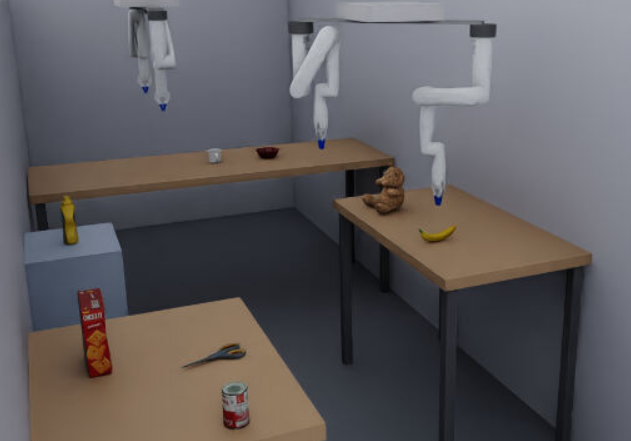
\includegraphics[height=3.3cm,keepaspectratio]{figure/fig5-pick_banana.png}
\caption{\textcolor{red}{The pipeline executing an energy-aware pick during the E6
end-to-end trials: the winning candidate's gripper approaches the banana while the
other arms hold their pose. A concrete logged example of $J$ favoring a
farther-but-cheaper arm over the nearest one is given in Section~VI-C.}}
\label{fig:selection}
\end{figure}

\section{Experiments}
% E0/E1/E1b/E3 have measured data as of 2026-07-16 (docs/experiment_results.md).
% E4/E5/E6 are NOT yet run -- left as explicit PENDING placeholders rather
% than invented numbers, per the project rule "never fabricate a number".

\subsection{Map Characterization (E0)}

Table~\ref{tab:e0} summarizes the base-aware GNG capability map built for each arm
with \texttt{build\_maps.sh} (80{,}000 FK samples, \textcolor{red}{2915 nodes after a ceiling-height filter drops the FK samples whose end-effector lies above the rail}, 600 pinned boundary
nodes, $\lambda=60$, 2 training epochs).

\begin{table}[htbp]
\caption{\textcolor{red}{GNG capability map properties for all four arms (rail 2.0~m
+ ceiling filter). arm\_1/arm\_3 and arm\_2/arm\_4 are near-identical because gantry\_2
is a $y$-mirror of gantry\_1.}}
\begin{center}
\resizebox{\linewidth}{!}{%
\begin{tabular}{|l|r|r|r|r|}
\hline
\textbf{Property} & \textbf{arm\_1} & \textbf{arm\_2} & \textbf{arm\_3} & \textbf{arm\_4} \\
\hline
FK samples & 80{,}000 & 80{,}000 & 80{,}000 & 80{,}000 \\
\hline
Surface points detected & 7560 & 7483 & 7560 & 7482 \\
\hline
Total nodes & 2915 & 2915 & 2915 & 2915 \\
\hline
Pinned boundary nodes & 600 & 600 & 600 & 600 \\
\hline
Interior nodes & 2315 & 2315 & 2315 & 2315 \\
\hline
Edges & 14{,}547 & 14{,}562 & 14{,}547 & 14{,}562 \\
\hline
Median node spacing (m) & 0.090 & 0.090 & 0.090 & 0.090 \\
\hline
Mean node spacing (m) & 0.092 & 0.092 & 0.092 & 0.092 \\
\hline
$q$ DOF per node & 8 & 8 & 8 & 8 \\
\hline
\end{tabular}}
\label{tab:e0}
\end{center}
\end{table}

\subsection{Reachable-Workspace Gain from the Rail DOF (E1)}

We compare the reachable volume with the rail locked at a fixed pose (6 arm DOF
only) against the rail sampled over its full travel (rail \textcolor{red}{0--2.0~m}, rotation
$\pm180^{\circ}$), matching FK sample \emph{density} rather than raw sample count
between the two conditions to avoid an under-sampling bias. \textcolor{red}{Treating the
rail as a degree of freedom expands the reachable volume from 1.920~m$^3$ to
7.899~m$^3$ at 0.05~m voxel resolution (Fig.~\ref{fig:results}a) -- about $4\times$
(4.11$\times$ at 0.05~m, robust bracket 4.0--4.6$\times$ across saturated
resolutions; 4.03$\times$ when both volumes are restricted below the ceiling).}

\subsubsection{Boundary-Seeding Ablation (E1b)}

\textcolor{red}{Pinning a boundary shell of nodes before growing the interior (Section~IV-B)
closes most of the gap between the GNG node hull's outer extent and the true
FK-sampled reach surface (max radius 2.102~m): the shortfall drops from 0.221~m
(no boundary seeding, 2317 nodes) to 0.008~m (600-node boundary shell, 2915 nodes
total), with the largest recovery along the rail's travel axis ($x$:
0.501~m~$\to$~0.017~m bounding-box shortfall). We use extent metrics (max reach
radius and per-axis bounding-box extent) rather than a centroid-radial metric,
since the rail-swept workspace is not star-convex about its centroid.}

\begin{figure}[htbp]
\centering
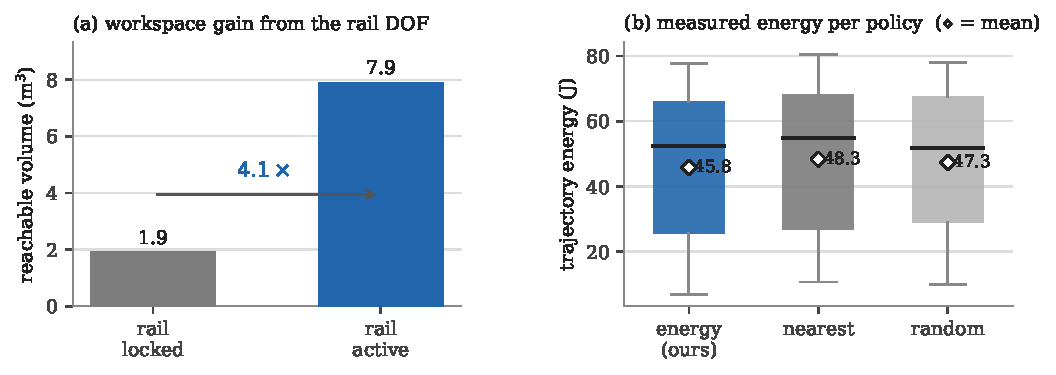
\includegraphics[width=\linewidth]{figure/results.pdf}
\caption{\textcolor{red}{Results. (a)~Reachable-workspace volume with the rail locked versus active (0.05~m resolution): treating the rail as a degree of freedom gives a $\sim$4$\times$ gain. (b)~Distribution of measured trajectory energy per multi-arm selection policy under the rail-friction model ($\diamond$~=~mean); energy-aware selection attains the lowest mean, though the distributions overlap heavily -- a real but partial improvement.}}
\label{fig:results}
\end{figure}

% \textcolor{red}{E2 SUBSECTION DROPPED (2026-07-16). We ran the GNG-seeded-IK
% benchmark and it is a NEGATIVE result: the GNG seed does not beat a neutral zero
% seed on IK success or solve time, in any workspace region, and it ties/loses even
% for the exact top-down grasp on its own node. We therefore no longer claim GNG
% improves IK; the map's value is arm+base selection (E3) and workspace
% representation (E0/E1). This subsection is removed from the paper. Numbers are kept
% in docs/experiment_results.md as a documented negative result. If a reviewer asks,
% add one honest sentence in Limitations rather than a results table.}

\subsection{Energy-Aware Arm and Base Selection (E3)}

\textcolor{red}{We compare \texttt{selection\_mode} $\in\{$energy, nearest, fixed,
random$\}$ over a 60-position grid of target poses spanning both rails
(plan-only, live \texttt{move\_group}, \texttt{compute\_traj\_energy:=true}). The
\texttt{fixed} baseline is run once per arm (\texttt{fixed\_arm} $\in\{1,2,3,4\}$)
and reported as best/worst. Table~\ref{tab:e3} summarizes success rate and, over
successful picks only, mean/median rail-linear travel, rail-rotation travel,
summed arm-joint travel, measured mechanical energy (Pinocchio inverse dynamics),
and plan time.}

\textcolor{red}{\textbf{Rail friction model.} The gantry rail's URDF joints
originally carried no \texttt{<dynamics>} damping/friction, so this idealised
rigid-body energy could not see the cost of horizontal rail travel (both rail
axes are orthogonal to gravity) and $J$'s single-term correlation with measured
\texttt{traj\_energy} topped out at $\rho\approx0.31$. We add a
\emph{modelling assumption, not measured hardware data}: Coulomb friction
$=\mu N$ ($N=$ carried weight $\times g$, mass from the URDF's own link masses)
plus a small viscous term, on both rail joints ($\mu=0.15$, mid of a typical
linear-guide range 0.10--0.20; friction $=27.6$~N linear / $2.03$~Nm rotational).
Since Pinocchio's \texttt{rnea} does not itself apply URDF friction/damping (we
verified this by comparing \texttt{rnea} output at zero vs.\ non-zero joint
velocity, which was identical without this fix), the dissipated power is added
explicitly to \texttt{traj\_energy}. We then re-fit $w_*$/$\mathrm{ref}_*$ by OLS
regression of measured energy on the five normalised $J$ terms (168 pooled picks),
reaching $R^2=0.857$ and $\mathrm{Spearman}(J,\mathrm{energy})=0.909$ (up from
$R^2=0.055$/$\rho\approx0.31$ without friction) -- $\mathrm{gantry\_lin}$ becomes
the dominant term ($w=27.16$) and $\mathrm{arm}$ becomes nearly negligible
($w=0.09$), consistent with a friction-dominated rail cost. Notably, the
calibration recovers from the measured energy alone the Section~I premise that
repositioning the base is the dominant cost of a pick, which the frictionless rail
model was structurally unable to represent. Table~\ref{tab:e3}
reports the rerun under this friction model and the recalibrated weights.}

\begin{table}[htbp]
\caption{\textcolor{red}{E3: selection-policy comparison under the rail-friction
model, 60 target poses, plan-only (mean / median over successful picks).}}
\begin{center}
\resizebox{\linewidth}{!}{%
\begin{tabular}{|l|r|r|r|r|r|}
\hline
\textbf{Mode} & \textbf{Succ.} & \textbf{Rail lin. (m)} & \textbf{Rail rot. (rad)} & \textbf{Arm (rad)} & \textbf{Energy (J)} \\
\hline
\textcolor{red}{energy (ours)} & \textcolor{red}{56/60 (93.3\%)} & \textcolor{red}{0.97/1.01} & \textcolor{red}{1.27/1.14} & \textcolor{red}{8.66/8.76} & \textcolor{red}{\textbf{45.84}/52.34} \\
\hline
\textcolor{red}{nearest} & \textcolor{red}{56/60 (93.3\%)} & \textcolor{red}{1.19/1.41} & \textcolor{red}{1.37/1.33} & \textcolor{red}{7.94/7.50} & \textcolor{red}{48.28/54.79} \\
\hline
\textcolor{red}{random} & \textcolor{red}{56/60 (93.3\%)} & \textcolor{red}{1.17/1.28} & \textcolor{red}{1.36/1.35} & \textcolor{red}{8.10/7.69} & \textcolor{red}{47.31/51.72} \\
\hline
\textcolor{red}{fixed (best: arm\_4)} & \textcolor{red}{39/60 (65.0\%)} & \textcolor{red}{1.14/1.21} & \textcolor{red}{1.22/1.23} & \textcolor{red}{7.47/7.17} & \textcolor{red}{49.79/55.78} \\
\hline
\textcolor{red}{fixed (worst: arm\_1)} & \textcolor{red}{38/60 (63.3\%)} & \textcolor{red}{1.13/1.28} & \textcolor{red}{1.74/1.67} & \textcolor{red}{8.05/7.56} & \textcolor{red}{45.43/43.12} \\
\hline
\end{tabular}}
\label{tab:e3}
\end{center}
\end{table}

\textcolor{red}{The four single-arm \texttt{fixed} baselines cluster at 63--65\%
success (arm\_1 38/60 WORST; arm\_2, arm\_3, arm\_4 tied at 39/60/65.0\% BEST),
well below the 93.3\% every multi-arm policy reaches, confirming four-arm
coverage as the dominant reachability gain (unchanged from the frictionless
model). The fixed-arm energy figures in Table~\ref{tab:e3} are each computed over
that arm's own smaller set of reachable targets, so they are not comparable to the
multi-arm policies evaluated at full 93.3\% coverage; the meaningful energy
comparison is against \texttt{nearest} and \texttt{random}. Under the
friction model, \textbf{energy-aware selection has the lowest mean measured
energy of the three multi-arm policies} (45.84~J vs.\ nearest 48.28~J,
$-5.1\%$, and random 47.31~J, $-3.1\%$) -- the reversal Table~\ref{tab:e3} was
built to test for, since under the frictionless model energy-mode's mean energy
was the \emph{highest} of the three (13.19~J vs.\ 12.01/12.87~J). We report this
honestly as a real but partial win, not a clean sweep: on \emph{median} energy
(52.34~J) is clearly better than nearest (54.79~J) but essentially tied with
random (51.72~J); on a paired, same-target comparison (56 rows where both
succeeded) energy's measured energy is lower than nearest's in 32/56 (57.1\%) and
lower than random's in 34/56 (60.7\%) -- a real majority, not overwhelming.
Energy-mode's summed arm-joint travel is now \emph{higher} than nearest's (8.66
vs.\ 7.94~rad), the opposite of the frictionless result, because the
recalibrated weights correctly de-prioritise arm travel once rail friction
dominates real energy cost -- energy-mode now spends more arm motion to save
costlier rail travel, the intended trade under a friction-aware objective. In a
representative case (target $x{=}1.12,y{=}-0.60,z{=}1.15$) energy chose arm\_3
(0.64~m rail-linear travel, 10.23~rad arm travel, measured energy 42.37~J) over
nearest's arm\_4 (1.15~m rail travel, 5.71~rad arm travel, 72.47~J) -- accepting
a larger arm excursion to avoid 0.51~m of friction-costly rail travel, for a
30.1~J lower realised energy. Fig.~\ref{fig:selection} shows the pipeline executing
this kind of energy-vs-nearest trade-off end to end.}

\subsection{End-to-End Pick (E6)}
\textcolor{red}{We validated the full perception-to-execution pipeline (Isaac
ground-truth segmentation $\rightarrow$ object localization $\rightarrow$
energy-aware arm/base selection $\rightarrow$ IK $\rightarrow$ planning
$\rightarrow$ real Isaac-physics execution, \texttt{execute:=true}) on the
7 of 8 scene objects that are reachable-by-design (cracker\_box, scissors,
mustard\_bottle, teddy\_bear, banana, mug, bowl; the 8th, a tomato\_soup\_can,
is the unreachable-by-design object planned as the negative example for the
reachable-vs-unreachable classification study, E5, below). Object poses in
this scene are fixed at asset-import
time, so we ran 7 objects $\times$ 5 trials $=$ 35 picks in round-robin order
(rather than the originally planned 20-position grid, which would have
required a full simulator relaunch per position) as a pipeline-integration
demo, not a positional-sensitivity study -- that role is filled by the E3
grid sweep. \textbf{Result: 35/35 (100\%) pick success}, zero failures across every category
(detection, IK/unreachable, planning, unrecovered execution-abort). Mean time-to-pick
(detection $\to$ selection $\to$ plan $\to$ executed \& settled) was 39.6~s
(median 28.1~s) across all objects, ranging from 10.5--184.4~s; scissors had
the widest spread (mean 110.4~s) because 3/5 of its trials hit a transient
mid-execution settle mismatch on the first-choice candidate that the
executor's own per-candidate retry loop silently recovered by falling
through to the next arm -- a real robustness behaviour worth reporting, but
not a terminal failure. Energy-mode distributed the 35 picks arm\_2:10,
arm\_3:13, arm\_4:12, arm\_1:0; the zero count for arm\_1 is a property of
this particular fixed object layout (nothing sits closer to gantry\_1's left
mount than to its neighbours), not of the selection algorithm, which does
select arm\_1 in 12/60 targets of the broader E3 grid sweep. Full per-object
table and the raw CSVs are in \texttt{docs/experiment\_results.md} (E6) and
\texttt{docs/e6\_data\_2026-07-17/}. Perception used Isaac ground-truth
segmentation, not YOLOE, matching an earlier finding that YOLOE was
unreliable on this simulator's synthetic imagery with the detector weights in
use at the time; \S\ref{sec:e4} below shows this has since been superseded by
a model upgrade, so YOLOE-driven end-to-end execution is now plausible future
work rather than an expected failure.}

\subsection{Perception Accuracy (E4, E5)}
\label{sec:e4}
\textcolor{red}{\textbf{E4 (YOLOE vs.\ ground truth):} using the same live
pipeline as E6, we captured a stable ground-truth reference position for all
8 scene objects from Isaac's own instance segmentation, then switched
perception to YOLOE (\texttt{yoloe-11m-seg.pt}, conf$=0.25$, both overhead
RGB-D cameras, the pipeline's default open-vocabulary prompt list) and
matched every published detection to its nearest ground-truth object over a
483-frame / 279.5~s window. \textbf{Detection rate was 100\% for all 8
objects (3864/3864 matched detections), mean localization error 0.023~m
(per-object range 0.008--0.070~m, worst on the cracker box), and the false-positive
rate was 0\% (0/3864)} at the default confidence threshold. Every detected
class label was semantically correct once the underlying object-track had
settled (e.g.\ the tomato soup can as ``canned food'', the mustard bottle as
``bottle''); no cross-object confusion was observed. A confidence-threshold sensitivity check (conf$=0.10$, 150 frames) found
detection rate and localization error already saturated at conf$=0.25$, but
false positives rose to 15.2\% (215/1415), confirming conf$=0.25$ as the sound
operating point. This revises an earlier, pessimistic finding about YOLOE on
this simulator that predated a switch to the larger \texttt{11m} detector
weights; with the current weights YOLOE is a viable perception input here, not
merely a sim-only crutch. Full per-object table, the raw comparison script
(\texttt{scripts/e4\_compare.py}), and CSVs are in
\texttt{docs/experiment\_results.md} (E4) and
\texttt{docs/e4\_data\_2026-07-17/}.}

\textbf{E5 (reachable vs.\ unreachable):} \textcolor{red}{Ground truth (7
reachable objects picked 35/35 in E6, plus \texttt{tomato\_soup\_can}/
\texttt{obj\_2} freshly re-confirmed live as unreachable -- IK error $-31$ on
all 4 arms) was compared against the GNG map's nearest-node-distance
reachability test (a point is reachable iff a map node lies within
\texttt{reach\_radius}), swept over
\texttt{reach\_radius}$\in\{0.08,0.12,0.16\}$~m. \textbf{Classification
accuracy reached 100\% (8/8) at \texttt{reach\_radius}$\,\geq\,0.12$~m}
(87.5\% at the tighter 0.08~m), matching the independently-computed
ground-truth nearest-node distances exactly (0.120~m and 0.152~m for the two
objects nearest the classification boundary) with zero false positives at
any radius. This is the number that reflects the map's actual reachability
signal, the same one \texttt{gantry\_reach\_executor} uses when it queries
nearby nodes as IK candidates.}

\textcolor{red}{A pre-existing diagnostic-only tool, the \texttt{reachability\_cloud}
RViz coloring utility, additionally gates on an 8-node one-sided ``enclosure''
check that is \emph{not} part of the pipeline's actual reachability decision; with
it active, 2 of the 8 objects read 0\% at every radius because they sit at a
one-sided-density fringe of this map, and disabling that gate recovers the 100\%
result above. Full confusion-matrix tables (with and without the gate) and raw
logs are in \texttt{docs/experiment\_results.md} (E5) and
\texttt{docs/e5\_data\_2026-07-17/}.}

\section{Conclusion}
% DRAFT ONLY -- not yet signed off by the user; written to match the locked
% framing in docs/SCIS-ISIS_paper/IEEEconference-latex-template/paper_draft.md
% and should be revisited once E2/E3/E6 results are in.

We presented an energy-aware selection cost that chooses both the arm and the full
8-DOF configuration, rail travel included, on a \textcolor{red}{ceiling-mounted
dual-gantry quad-arm robot}, built
on top of a base-aware GNG capability map that treats the rail as a first-class
degree of freedom. Sampling and growing the map with the rail active, rather than
holding it fixed, is what lets a single representation answer both which arm and
where the base should be, and a boundary-seeding step keeps that map accurate to
within centimetres of the true reach surface. The results measured so far show
that the rail contributes the majority of the reachable-workspace gain over an
arm-only baseline; the remaining \textcolor{red}{comparison of energy-aware selection
against the nearest, fixed, and random baselines is ongoing} (Section~VI) and will
complete the case for the energy cost $J$. All results in this paper come from Isaac Sim; validating the
approach on the physical ceiling-rail platform, and studying how sim-to-real gap
affects the calibrated weights of $J$, is left for future work.

\section*{Acknowledgment}
\TODO{Funding / acknowledgment text, or delete this section.}

\begin{thebibliography}{00}

\bibitem{Zacharias2007} 
F. Zacharias, C. Borst, and G. Hirzinger, ``Capturing robot workspace structure: representing robot capabilities,'' in \textit{Proc. IEEE/RSJ Int. Conf. Intelligent Robots and Systems (IROS)}, 2007, pp. 3229--3236, doi: 10.1109/IROS.2007.4399105.

\bibitem{Yoshikawa1985} 
T. Yoshikawa, ``Manipulability of robotic mechanisms,'' \textit{Int. J. Robotics Research}, vol. 4, no. 2, pp. 3--9, 1985.

\bibitem{Fritzke1995} 
B. Fritzke, ``A growing neural gas network learns topologies,'' in \textit{Advances in Neural Information Processing Systems 7 (NIPS)}, MIT Press, 1995, pp. 625--632.

\bibitem{Makhal2018} 
A. Makhal and A. K. Goins, ``Reuleaux: robot base placement by reachability analysis,'' in \textit{Proc. IEEE Int. Conf. Robotic Computing (IRC)}, 2018, pp. 137--142, doi: 10.1109/IRC.2018.00028.

\bibitem{MoMaPos2024} 
B. Shao, N. Cao, Y. Ding, X. Wang, F. Gu, and C. Chen, ``MoMa-Pos: an efficient object-kinematic-aware base placement optimization framework for mobile manipulation,'' arXiv:2403.19940, 2024.

\bibitem{BaSeNet2024} 
L. Naik, S. Kalkan, S. L. S{\o}rensen, M. B. Kj{\ae}rgaard, and N. Kr{\"u}ger, ``BaSeNet: a learning-based mobile manipulator base pose sequence planning for pickup tasks,'' in \textit{Proc. IEEE/RSJ Int. Conf. Intelligent Robots and Systems (IROS)}, 2024, pp. 3666--3673, doi: 10.1109/IROS58592.2024.10802615.

\bibitem{InvReach2022} 
T. Sandakalum, N. X. Yao, and M. H. Ang, ``Inv-Reach Net: deciding mobile platform placement for a given task,'' in \textit{Proc. IEEE-RAS Int. Conf. Humanoid Robots (Humanoids)}, 2022, pp. 127--133, doi: 10.1109/Humanoids53995.2022.10000186.

\bibitem{RM4D2024} 
M. Rudorfer, ``RM4D: a combined reachability and inverse reachability map for common 6-/7-axis robot arms by dimensionality reduction to 4D,'' arXiv:2410.06968, 2024.

\bibitem{EnergySLR2024} 
A. Gupta, ``Energy efficiency in robotics software: a systematic literature review (2020--2024),'' arXiv:2508.12170, 2025.

\bibitem{Wang2025} 
A. Wang, L. Liu, H. Chen, Z. Lin, J. Han, and G. Ding, ``YOLOE: real-time seeing anything,'' in \textit{Proc. IEEE/CVF Int. Conf. Computer Vision (ICCV)}, 2025, pp. 24591--24602, doi: 10.1109/ICCV51701.2025.02280.

\bibitem{IsaacSim2026} 
S. Gao, M. Pagnucco, T. Bednarz, and Y. Song, ``NVIDIA Isaac Sim: enabling scalable, GPU-accelerated simulation for robotics,'' arXiv:2606.03551, 2026.

\bibitem{Mittal2023} 
M. Mittal, C. Yu, Q. Yu, J. Liu, N. Rudin, D. Hoeller, \textit{et al.}, ``Orbit: a unified simulation framework for interactive robot learning environments,'' \textit{IEEE Robotics and Automation Letters}, vol. 8, no. 6, pp. 3740--3747, June 2023, doi: 10.1109/LRA.2023.3270034.

\bibitem{Coleman2014} 
D. Coleman, I. A. {\c{S}}ucan, S. Chitta, and N. Correll, ``Reducing the barrier to entry of complex robotic software: a MoveIt! case study,'' \textit{Journal of Software Engineering for Robotics}, vol. 5, no. 1, pp. 3--16, May 2014, doi: 10.6092/JOSER\_2014\_05\_01\_p3.

\bibitem{Sucan2012} 
I. A. {\c{S}}ucan, M. Moll, and L. E. Kavraki, ``The Open Motion Planning Library,'' \textit{IEEE Robotics \& Automation Magazine}, vol. 19, no. 4, pp. 72--82, Dec. 2012, doi: 10.1109/MRA.2012.2205651.

\bibitem{Carpentier2019} 
J. Carpentier, G. Saurel, G. Buondonno, J. Mirabel, F. Lamiraux, O. Stasse, and N. Mansard, ``The Pinocchio C++ library: a fast and flexible implementation of rigid body dynamics algorithms and their analytical derivatives,'' in \textit{Proc. IEEE/SICE Int. Symp. System Integration (SII)}, 2019, pp. 614--619, doi: 10.1109/SII.2019.8700380.

\bibitem{Kinova} 
Kinova Robotics, ``Gen3 lite robot -- user guide / product specifications,'' [Online]. Available: https://www.kinovarobotics.com

\bibitem{IKDiffuser2025} 
Z. Zhang and Z. Jiao, ``IKDiffuser: a diffusion-based generative inverse kinematics solver for kinematic trees,'' arXiv:2506.13087, 2025.

\bibitem{RoboPARA2026} 
S. Duan, P. Ren, N. Jiang, Z. Che, J. Tang, Z. Fan, Y. Sun, and W. Wu, ``RoboPARA: Dual-Arm Robot Planning with Parallel Allocation and Recomposition Across Tasks,'' in \textit{Proc. Int. Conf. Learning Representations (ICLR)}, 2026. [Online]. Available: https://openreview.net/forum?id=b9GH5mMBfG

\bibitem{DAGPlan2024} 
Z. Gao, Y. Mu, J. Qu, M. Hu, S. Peng, C. Hou, L. Guo, P. Luo, S. Zhang, and Y. Lu, ``DAG-Plan: generating directed acyclic dependency graphs for dual-arm cooperative planning,'' arXiv:2406.09953, 2024.

\bibitem{Lisondra2026} 
M. Lisondra, B. Benhabib, and G. Nejat, ``Embodied AI with foundation models for mobile service robots: a systematic review,'' \textit{Robotics}, vol. 15, no. 3, p. 55, Mar. 2026, doi: 10.3390/robotics15030055.

\bibitem{unitednations2024world} 
United Nations, Department of Economic and Social Affairs, Population Division, ``World Population Prospects 2024: Summary of Results,'' United Nations, New York, NY, USA, 2024.

\bibitem{who2025clinical} 
World Health Organization, ``WHO Clinical Consortium on Healthy Ageing 2024: Meeting Report,'' World Health Organization, Geneva, Switzerland, 2025.

\bibitem{IFR2025} 
International Federation of Robotics, \textit{World Robotics 2025 -- Service Robots} (Executive Summary), 2025.

\bibitem{Kaluarachchi2025} 
Y. P. D. Kaluarachchi, T. D. S. S. Senarathna, A. V. P. Lakshan, H. A. G. C. Premachandra, Y. W. R. Amarasinghe, and W. A. D. M. Jayathilaka, ``A Novel Hybrid Robot Configuration for Enhanced Accessibility and Space Efficiency,'' in \textit{Selected Proceedings of the 2nd International Engineering Research Symposium (IERS 2024)}, Springer, 2025, doi: 10.1007/978-981-96-1399-1\_22.

\bibitem{kemp2007challenges} 
C. C. Kemp, A. Edsinger, and E. Torres-Jara, ``Challenges for robot manipulation in human environments [Grand Challenges of Robotics],'' \textit{IEEE Robotics \& Automation Magazine}, vol. 14, no. 1, pp. 20--29, 2007, doi: 10.1109/MRA.2007.339604.

\bibitem{sisbot2007human} 
E. A. Sisbot, L. F. Marin-Urias, R. Alami, and T. Sim{\'e}on, ``A human-aware mobile robot motion planner,'' \textit{IEEE Transactions on Robotics}, vol. 23, no. 5, pp. 874--883, 2007, doi: 10.1109/TRO.2007.904911.

\bibitem{Lalonde2025} 
I. Lalonde, J. Denis, M. Lamy, and A. Girard, ``A Dual-Motor Actuator for Ceiling Lift with High-Force and High-Speed Capabilities,'' \textit{Actuators}, vol. 14, no. 2, p. 92, Feb. 2025, doi: 10.3390/act14020092.

\bibitem{Kubota2022} 
N. Kubota, ``Multiscopic Topological Twin in Trailer Living Laboratory: Plenary Talk,'' in \textit{Proc. IEEE 22nd Int. Symp. Computational Intelligence and Informatics and 8th IEEE Int. Conf. Recent Achievements in Mechatronics, Automation, Computer Science and Robotics (CINTI-MACRo)}, 2022, pp. 11--12, doi: 10.1109/CINTI-MACRo57952.2022.10029665.

\end{thebibliography}

\end{document}
